\documentclass[11pt,a4paper]{article}
\usepackage[utf8]{inputenc}
\usepackage[vietnamese]{babel}
\usepackage{amsmath,amssymb}
\usepackage[version=4]{mhchem}
\usepackage{geometry}
\geometry{top=1.5cm,bottom=1.2cm,left=1.4cm,right=1.4cm,headheight=28pt,headsep=12pt,footskip=18pt}
\usepackage{graphicx}
\usepackage{xcolor}
\usepackage{tabularx}
\usepackage{array}
\usepackage{colortbl}
\usepackage{tikz}
\usepackage{chemfig}
\usepackage{fancyhdr}
\usepackage{enumitem}
\usepackage{multido}
\usepackage{tcolorbox}

\definecolor{hfRed}{HTML}{D32F2F}
\definecolor{hfGreen}{HTML}{8BC390}
\definecolor{mainGreen}{HTML}{2E7D32}
\definecolor{solBlue}{HTML}{1565C0}
\definecolor{tableGreen}{HTML}{E8F5E9}

\usepackage{ex_test}

\pagestyle{fancy}
\fancyhf{}
\renewcommand{\headrulewidth}{0.75pt}
\renewcommand{\headrule}{\hbox to\headwidth{\color{hfGreen}\leaders\hrule height \headrulewidth\hfill}}
\renewcommand{\footrulewidth}{0.75pt}
\renewcommand{\footrule}{\hbox to\headwidth{\color{hfGreen}\leaders\hrule height \footrulewidth\hfill}}

\fancyhead[L]{\small\itshape\color{hfRed}Tài liệu lưu hành nội bộ}
\fancyhead[R]{\small\color{hfRed}Thầy \textbf{TRẦN VĂN THẠNH} - 0777.470.803}

\fancyfoot[L]{\footnotesize\itshape\color{hfRed}CS1: 6/15 Nguyễn Hoàng, P. Kim Long, TP Huế \quad|\quad CS2: 24 Đặng Thái Thân, TP Huế}
\fancyfoot[R]{\small\textbf{\color{hfRed}Trang \thepage}}

\setlength{\parindent}{0pt}
\setlength{\parskip}{2pt}

\begin{document}

\begin{minipage}[t]{0.48\textwidth}
\textbf{SỞ GD - ĐT THÀNH PHỐ HUẾ}\\
\textbf{TRƯỜNG THPT ĐẶNG HUY TRỨ}\\
\textit{ĐỀ CHÍNH THỨC}\\
\textit{(Đề thi có 03 trang)}
\end{minipage}
\hfill
\begin{minipage}[t]{0.48\textwidth}
\raggedleft
\textbf{\color{hfRed}KIỂM TRA CUỐI KỲ I}\\
\textbf{NĂM HỌC 2025 -- 2026}\\
\textbf{MÔN: HÓA HỌC -- LỚP 11}\\
\textit{Thời gian làm bài: 45 phút (không kể thời gian phát đề)}\\
\textbf{MÃ ĐỀ: 102}
\end{minipage}

\vspace{4pt}
\noindent
\textit{Họ và tên học sinh:} \dotfill \textit{Lớp:} \dotfill \textit{SBD:} \dotfill

\vspace{3pt}
\noindent
\textit{\footnotesize Cho biết nguyên tử khối của các nguyên tố: $\ce{C} = 12; \ce{H} = 1; \ce{O} = 16; \ce{Ba} = 137; \ce{S} = 32$.}

\vspace{3pt}
\hrule color{hfGreen} height 0.5pt

\vspace{6pt}
{\large\bfseries\color{mainGreen} A. TRẮC NGHIỆM (7,0 điểm)}

\vspace{3pt}
{\bfseries\color{mainGreen} Phần I: Trắc nghiệm nhiều lựa chọn (4,0 điểm).}
\textit{Học sinh trả lời từ câu 1 đến câu 16. Mỗi câu hỏi học sinh chỉ chọn một phương án.}
\vspace{4pt}
\begin{ex}
Công thức phân tử chất hữu cơ \textbf{không thể} cho ta biết:
\choice
{Tỉ lệ giữa các nguyên tố trong hợp chất}
{Số lượng các nguyên tố trong hợp chất.}
{Cấu trúc phân tử hợp chất hữu cơ.}
{Hàm lượng mỗi nguyên tố trong hợp chất.}
\loigiai{}
\end{ex}
\begin{ex}
Cho phổ khối lượng của một hợp chất hữu cơ A như hình vẽ:
\begin{center}
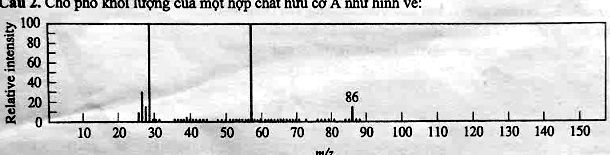
\includegraphics[width=0.75\textwidth]{images_danghuytru_ma102/ms_cau2_clean.png}
\end{center}
Hợp chất hữu cơ A có thể là
\choice
{\ce{C4H8O2}.}
{\ce{CH2Cl2}.}
{\ce{C4H6O2}.}
{\ce{C7H8}.}
\loigiai{}
\end{ex}
\begin{ex}
Dung dịch nào sau đây có $\text{pH} \approx 7$?
\choice
{\ce{NaOH}.}
{\ce{NaCl}.}
{\ce{HNO3}.}
{\ce{H2SO4}.}
\loigiai{}
\end{ex}
\begin{ex}
Khi phản ứng với kim loại, Sulfur thể hiện tính chất gì?
\choice
{tính khử.}
{tính lưỡng tính.}
{tính oxi hóa.}
{vừa tính oxi hóa, vừa tính khử.}
\loigiai{}
\end{ex}
\begin{ex}
Phú dưỡng là hiện tượng môi trường nước (ao, hồ, sông) bị dư thừa quá mức các chất dinh dưỡng, chủ yếu là Nitơ (N) và Photpho (P), do nước thải nông nghiệp, sinh hoạt, công nghiệp đổ vào, dẫn đến sự phát triển bùng nổ của tảo (nở hoa) và vi sinh vật, gây thiếu oxy, chết cá, làm suy giảm chất lượng nước và mất cân bằng sinh thái.

Cách nào sau đây \textbf{không đúng} khi xử lí hiện tượng phú dưỡng trong các ao hồ?
\choice
{Sử dụng phân bón hợp lý trong nông nghiệp.}
{Phun thuốc diệt cỏ để diệt tảo.}
{Xử lý nước thải trước khi xả ra môi trường.}
{Nạo vét bùn, khơi thông dòng chảy cho ao, hồ, sông.}
\loigiai{}
\end{ex}
\begin{ex}
Để tách các chất lỏng ra khỏi hỗn hợp các chất có nhiệt độ sôi khác nhau, nhằm thu được chất lỏng tinh khiết hơn là phương pháp nào sau đây?
\choice
{Phương pháp chưng cất.}
{Phương pháp chiết}
{Sắc kí cột.}
{Phương pháp kết tinh.}
\loigiai{}
\end{ex}
\begin{ex}
\ce{HNO3} tinh khiết là chất lỏng không màu, nhưng dung dịch \ce{HNO3} để lâu thường chuyển sang màu vàng là do
\choice
{khi để lâu thì \ce{HNO3} bị khử bởi các chất của môi trường}
{dung dịch \ce{HNO3} có hoà tan một lượng nhỏ \ce{NO2}.}
{dung dịch \ce{HNO3} có tính oxi hoá mạnh.}
{\ce{HNO3} tan nhiều trong nước.}
\loigiai{}
\end{ex}
\begin{ex}
Phản ứng hóa học của các hợp chất hữu cơ có đặc điểm là:
\choice
{thường xảy ra rất nhanh và cho một sản phẩm duy nhất.}
{thường xảy ra rất chậm, nhưng hoàn toàn, không theo một hướng xác định.}
{thường xảy ra rất nhanh, không hoàn toàn, không theo một hướng nhất định.}
{thường xảy ra chậm, không hoàn toàn, không theo một hướng nhất định.}
\loigiai{}
\end{ex}
\begin{ex}
Trong các phát biểu sau đây, phát biểu nào \textbf{đúng} khi một hệ ở trạng thái cân bằng?
\choice
{Nồng độ của các chất trong hệ không đổi.}
{Phản ứng thuận đã dừng.}
{Nồng độ chất tham gia và sản phẩm bằng nhau.}
{Phản ứng nghịch đã dừng.}
\loigiai{}
\end{ex}
\begin{ex}
Tính chất nào sau đây \textbf{không phải} tính chất của dung dịch sulfuric acid đặc?
\choice
{Tính háo nước.}
{Tính oxi hóa.}
{Tính acid.}
{Tính khử.}
\loigiai{}
\end{ex}
\begin{ex}
Phát biểu nào sau đây \textbf{đúng} khi nói về sự điện li?
\choice
{Sự điện li thực chất là quá trình oxi hoá – khử.}
{Sự điện li quá trình hòa tan một chất vào nước tạo thành dung dịch.}
{Sự điện li quá trình phân li một chất dưới tác dụng của dòng điện.}
{Sự điện li là quá trình phân li một chất trong nước thành ion.}
\loigiai{}
\end{ex}
\begin{ex}
Xác định công thức cấu tạo thu gọn của hợp chất sau:
\begin{center}
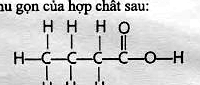
\includegraphics[width=0.35\textwidth]{images_danghuytru_ma102/ctct_cau12_clean.png}
\end{center}
\choice
{\ce{CH3CH2CH2COOH}.}
{\ce{CH3CH2CH2OH}.}
{\ce{CH3CH2CHOHCHO}.}
{\ce{CH3CH2COOH}.}
\loigiai{}
\end{ex}
\begin{ex}
Cho chất X có công thức cấu tạo thu gọn như sau: $\ce{CH3-COOH}$. Phân tử chất X chứa nhóm chức gì?
\choice
{-COO-}
{-CO-}
{-CHO}
{-COOH}
\loigiai{}
\end{ex}
\begin{ex}
Liên kết hoá học trong phân tử \ce{NH3} là liên kết
\choice
{cộng hoá trị có cực.}
{phối trí.}
{cộng hoá trị không cực.}
{ion.}
\loigiai{}
\end{ex}
\begin{ex}
Cho dung dịch \ce{HNO3} tác dụng với các chất sau: \ce{NH3}, \ce{CaCO3}, \ce{Ag}, \ce{NaOH}. Theo Bronsted, số phản ứng trong đó \ce{HNO3} đóng vai trò acid là
\choice
{1.}
{4.}
{3.}
{2.}
\loigiai{}
\end{ex}
\begin{ex}
Glucose là hợp chất hữu cơ có nhiều trong các loại quả chín, đặc biệt là quả nho. Công thức phân tử của glucose là \ce{C6H12O6}. Công thức đơn giản nhất của glucose là
\choice
{\ce{CHO2}.}
{\ce{CH3O}.}
{\ce{C3H4O3}.}
{\ce{CH2O}.}
\loigiai{}
\end{ex}

\vspace{6pt}
{\bfseries\color{mainGreen} Phần II: Trắc nghiệm dạng Đúng/Sai (2,0 điểm).}
\textit{Học sinh trả lời từ câu 1 đến câu 2. Trong mỗi ý a), b), c), d) ở mỗi câu, học sinh chọn đúng hoặc sai.}
\vspace{4pt}
\begin{ex}
Sulfur dioxide ($\ce{SO2}$) là một chất khí không màu, có mùi hăng đặc trưng, nặng hơn không khí và có mặt trong không khí từ các nguồn khác nhau.
\choiceTF
{ Khí $\ce{SO2}$ là một trong những tác nhân gây ô nhiễm môi trường và viêm đường hô hấp ở người, ...}
{ Để giảm thải $\ce{SO2}$ vào khí quyển cần xử lí khí thải công nghiệp, sử dụng các nhiên liệu sinh học và năng lượng tái tạo thay cho nhiên liệu hóa thạch.}
{ Cùng với khí $\ce{NO2}$, khí $\ce{SO2}$ là nguyên nhân chính gây nên hiện tượng mưa acid.}
{ Nguồn phát sinh $\ce{SO2}$ hiện tượng sấm sét trong khí quyển tạo nên.}
\loigiai{}
\end{ex}
\begin{ex}
Cho một số công thức cấu tạo của các chất như sau:
\begin{center}
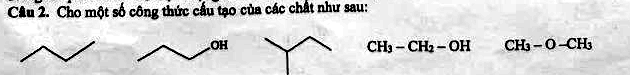
\includegraphics[width=0.85\textwidth]{images_danghuytru_ma102/structures_p2_c2_clean.png}
\end{center}
\choiceTF
{ Công thức cấu tạo (2) và (4) biểu diễn cùng một chất.}
{ Chất (2) và (4) có tính chất hoá học tương tự nhau.}
{ Chất (4) và (5) là đồng phân của nhau.}
{ Chất (1) và (3) là hydrocarbon mạch hở không phân nhánh..}
\loigiai{}
\end{ex}

\vspace{6pt}
{\bfseries\color{mainGreen} Phần III: Trắc nghiệm trả lời ngắn (1,0 điểm).}
\textit{Học sinh trả lời từ câu 1 đến câu 4.}
\vspace{4pt}
\begin{ex}
Cho 6 hợp chất hữu cơ có công thức phân tử lần lượt là: $\ce{C2H6O}$, $\ce{C2H4O2}$, $\ce{C3H6O3}$, $\ce{C3H6O2}$, $\ce{C4H8O2}$, $\ce{C6H12O6}$. Có bao nhiêu hợp chất hữu cơ \textbf{không có} công thức đơn giản nhất là $\ce{CH2O}$?
\par\textit{Trả lời:} \dotfill
\loigiai{}
\end{ex}
\begin{ex}
Trộn 200 mL dung dịch gồm $\ce{HCl}$ 0,1M và $\ce{H2SO4}$ 0,05M vào 300 mL dung dịch $\ce{Ba(OH)2}$ có nồng độ $a\text{ mol/L}$ thu được có $\text{pH} = 13$. Giá trị của $a$ là \textit{(Kết quả làm tròn đến hàng phần trăm)}.
\par\textit{Trả lời:} \dotfill
\loigiai{}
\end{ex}
\begin{ex}
Các cách làm sau đây, cách nào sử dụng phương pháp chiết?
\begin{enumerate}[label=(\arabic*),leftmargin=20pt,itemsep=0pt]
\item Giã lá cây chàm, cho vào nước, lọc lấy dung dịch màu để nhuộm sợi, vải.
\item Dùng nước sôi để pha trà, cà phê.
\item Ngâm rượu thuốc.
\item Làm đường cát, đường phèn từ nước mía.
\end{enumerate}
\par\textit{Trả lời:} \dotfill
\loigiai{}
\end{ex}
\begin{ex}
Có một loại quặng pyrite chứa 84\% $\ce{FeS2}$. Nếu mỗi ngày nhà máy sản xuất 10 tấn sulfuric acid 98\% thì cần $m$ tấn quặng pyrite trên và biết hiệu suất của cả quá trình sản xuất $\ce{H2SO4}$ là 60\%. Giá trị của $m$ là \textit{(Kết quả làm tròn đến hàng phần mười)}.
\par\textit{Trả lời:} \dotfill
\loigiai{}
\end{ex}

\vspace{6pt}
{\large\bfseries\color{mainGreen} B. TỰ LUẬN (3,0 điểm)}

\vspace{3pt}
\textbf{Câu 1 (1,0 điểm):} Hoàn thành phương trình hóa học của các phản ứng sau?
\begin{enumerate}[label=\alph*),leftmargin=25pt,itemsep=2pt]
\item $\ce{KOH + H2SO4 ->}$
\item $\ce{H2SO4\text{ loãng} + Fe2O3 ->}$
\item $\ce{NO2 + O2 + H2O ->}$
\item $\ce{NH4Cl + NaOH ->}$
\end{enumerate}

\vspace{2pt}
\multido{}{6}{\noindent\dotfill\par\vspace{2pt}}

\vspace{4pt}
\textbf{Câu 2 (1,0 điểm):} Camphor (có trong cây long não) là một chất rắn kết tinh màu trắng hay trong suốt giống như sáp với mùi thơm đặc trưng, thường dùng trong y học. Phần trăm khối lượng các nguyên tố trong camphor lần lượt là 78,94\% carbon, 10,53\% hydrogen và 10,53\% oxygen.

\begin{minipage}[t]{0.52\textwidth}
1) Lập công thức đơn giản nhất của camphor.\\
b) Xác định công thức phân tử của camphor biết phổ MS của camphor được cho như hình bên.
\end{minipage}
\hfill
\begin{minipage}[t]{0.45\textwidth}
\centering
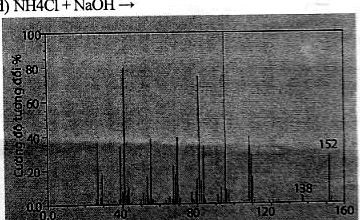
\includegraphics[width=0.95\textwidth]{images_danghuytru_ma102/ms_camphor_clean.png}
\end{minipage}

\vspace{2pt}
\multido{}{8}{\noindent\dotfill\par\vspace{2pt}}

\vspace{4pt}
\textbf{Câu 3 (1,0 điểm):} Hàm lượng cho phép của sulfur trong nhiên liệu là 0,3\% về khối lượng. Để xác định hàm lượng sulfur trong một loại nhiên liệu người ta lấy 100,0 gam nhiên liệu đó và đốt cháy hoàn toàn. Khí tạo thành chỉ chứa carbon dioxide, sulfur dioxide và hơi nước được dẫn vào nước tạo ra 500,0 ml dung dịch. Biết rằng tất cả sulfur dioxide đã tan vào dung dịch. Lấy 10,0 ml dung dịch này cho tác dụng với dung dịch $\ce{KMnO4}\ 5{,}00\cdot 10^{-3}\text{ mol/L}$ thì thể tích dung dịch $\ce{KMnO4}$ cần dùng là 12,5 mL. Tính phần trăm khối lượng của sulfur trong nhiên liệu trên?\\
\textit{(Cho NTK các nguyên tố: C: 12, H: 1, O: 16, Ba: 137, S: 32)}

\vspace{2pt}
\multido{}{10}{\noindent\dotfill\par\vspace{2pt}}

\vspace{6pt}
\begin{center}
\textbf{\large ---------- HẾT ----------}
\end{center}

\end{document}
